\section{Look Ahead}
\subsection{Theory of Operation}

The look ahead node is responsible for obstacle detection. The node
subscribes to lidar data and uses trigonometric functions to check for
obstacles within a bounded box.  The box's dimensions are currently 1m
in front of the robot and .25m on either side. 

The node constantly publishes to the obstacles topic using a custom
message type of ``Obstacle''.  The Obstacle message and the
subscribers of the obstacle topic are described in Custom Message
Specifications section.

In order to perform its job the Look Ahead node subscribes to the
lidar data published with message type sensor\_msgs/laserscan. This message
includes information about each laser ping's distance and intensity as
well as information about the laser range finder device itself.  In
our case, the lidar is set to do 181 pings on every sweep with spacing
of 1 degree per ping.  This works out to a sweep from -90$^\circ$ to
90$^\circ$ in the robots base coordinate frame.

When an obstacle is detected in the box the obstacles boolean in the
Obstalce message type is set to true. The algorithm also calculates
the closest of the obstacle pings and puts that number in the distance field
of the Obstacle message type. When no obstacles are detected obstacles
is set to false and distance is set to 0.0.

\subsubsection{Implementation Decisions}

To account for the possibility of more pings per sweep or sweeps of
smaller degrees we have constants that are defined globally at the top
of the file.  This gives us a single place to change fundamental
parameters of the program.  We could potentially move these into a
configuration file to prevent the need to recompile when new settings
are desired.

\subsubsection{Bounding Box Algorithm}
To determine if a ping is within the box dimensions the trigonemetric
functions are used to determine the bounds of the box.  For each ping
a maximum distance is computed.  If the ping distance is larger than this
value then it is ignored. If the ping distance is less it is
considered an obstacle.  The minimum of all pings within the distance
thresholds is returned as the distance.

\FloatBarrier
\begin{figure}[h]
  \centering
  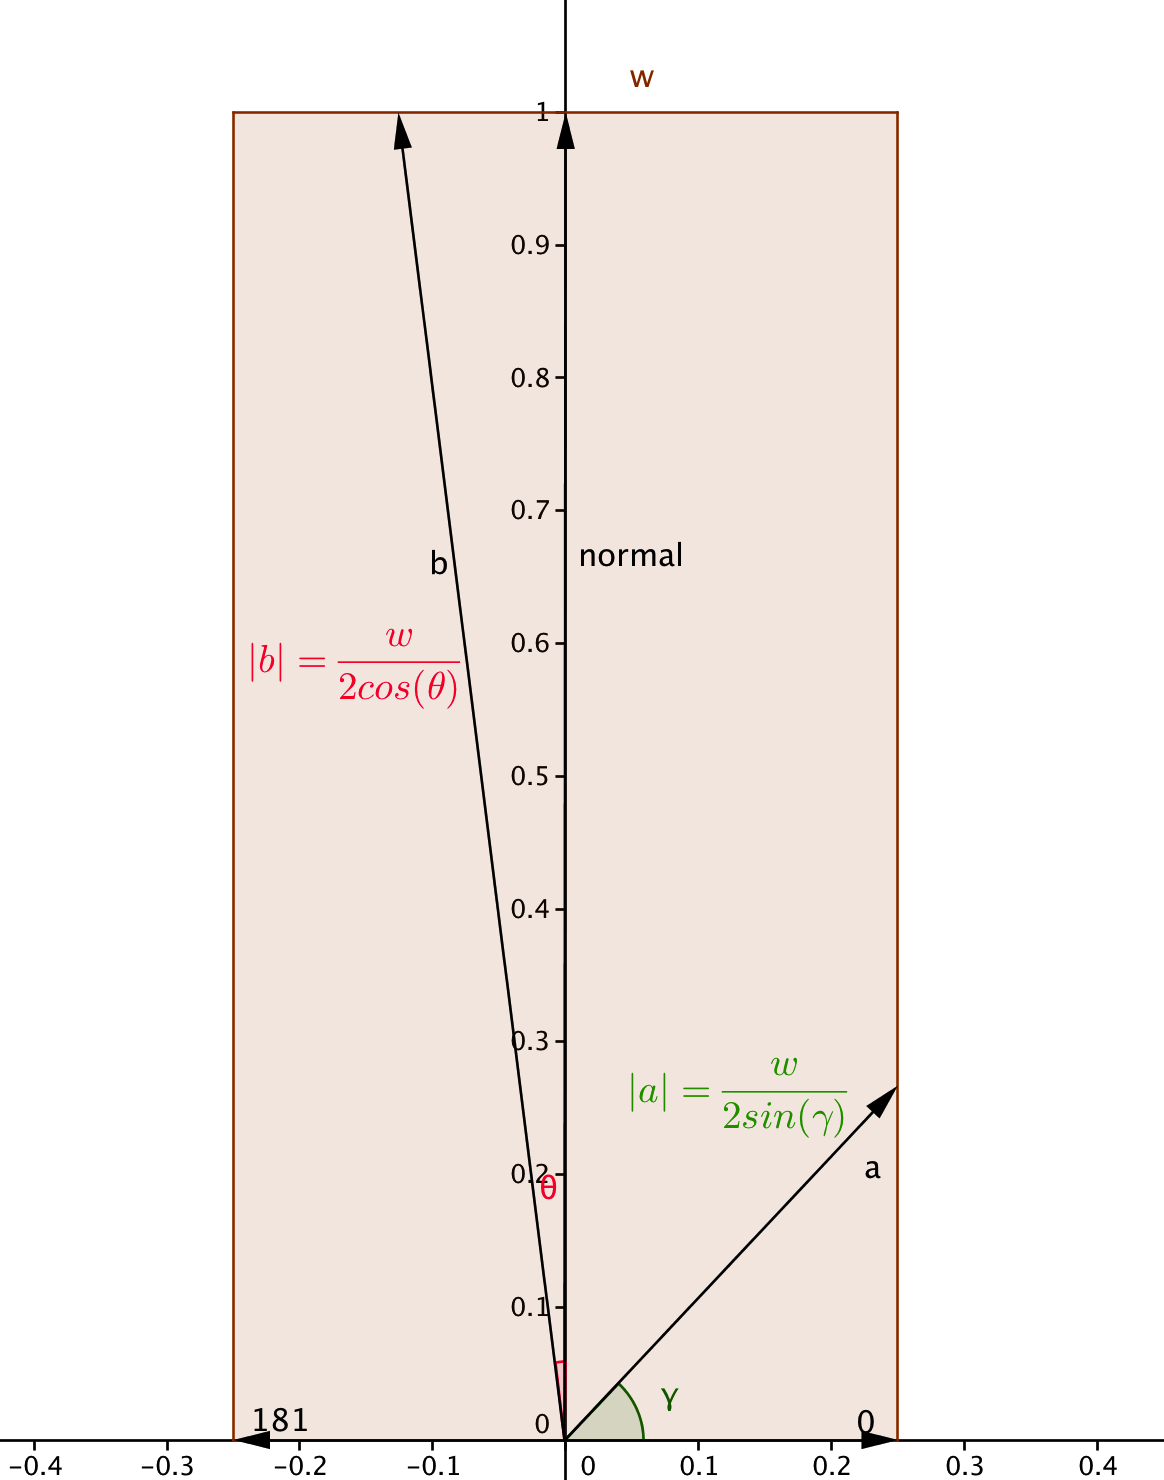
\includegraphics[height=4.5in]{Look_Ahead_Bounding_Box.png}
  \caption{Calculations for laser ping distances}
\end{figure}
\FloatBarrier

In this figure a laser ping from each of the two region types is shown
along with the function used to calculate the maximum distance.

\FloatBarrier
\begin{figure}[h]
  \centering
  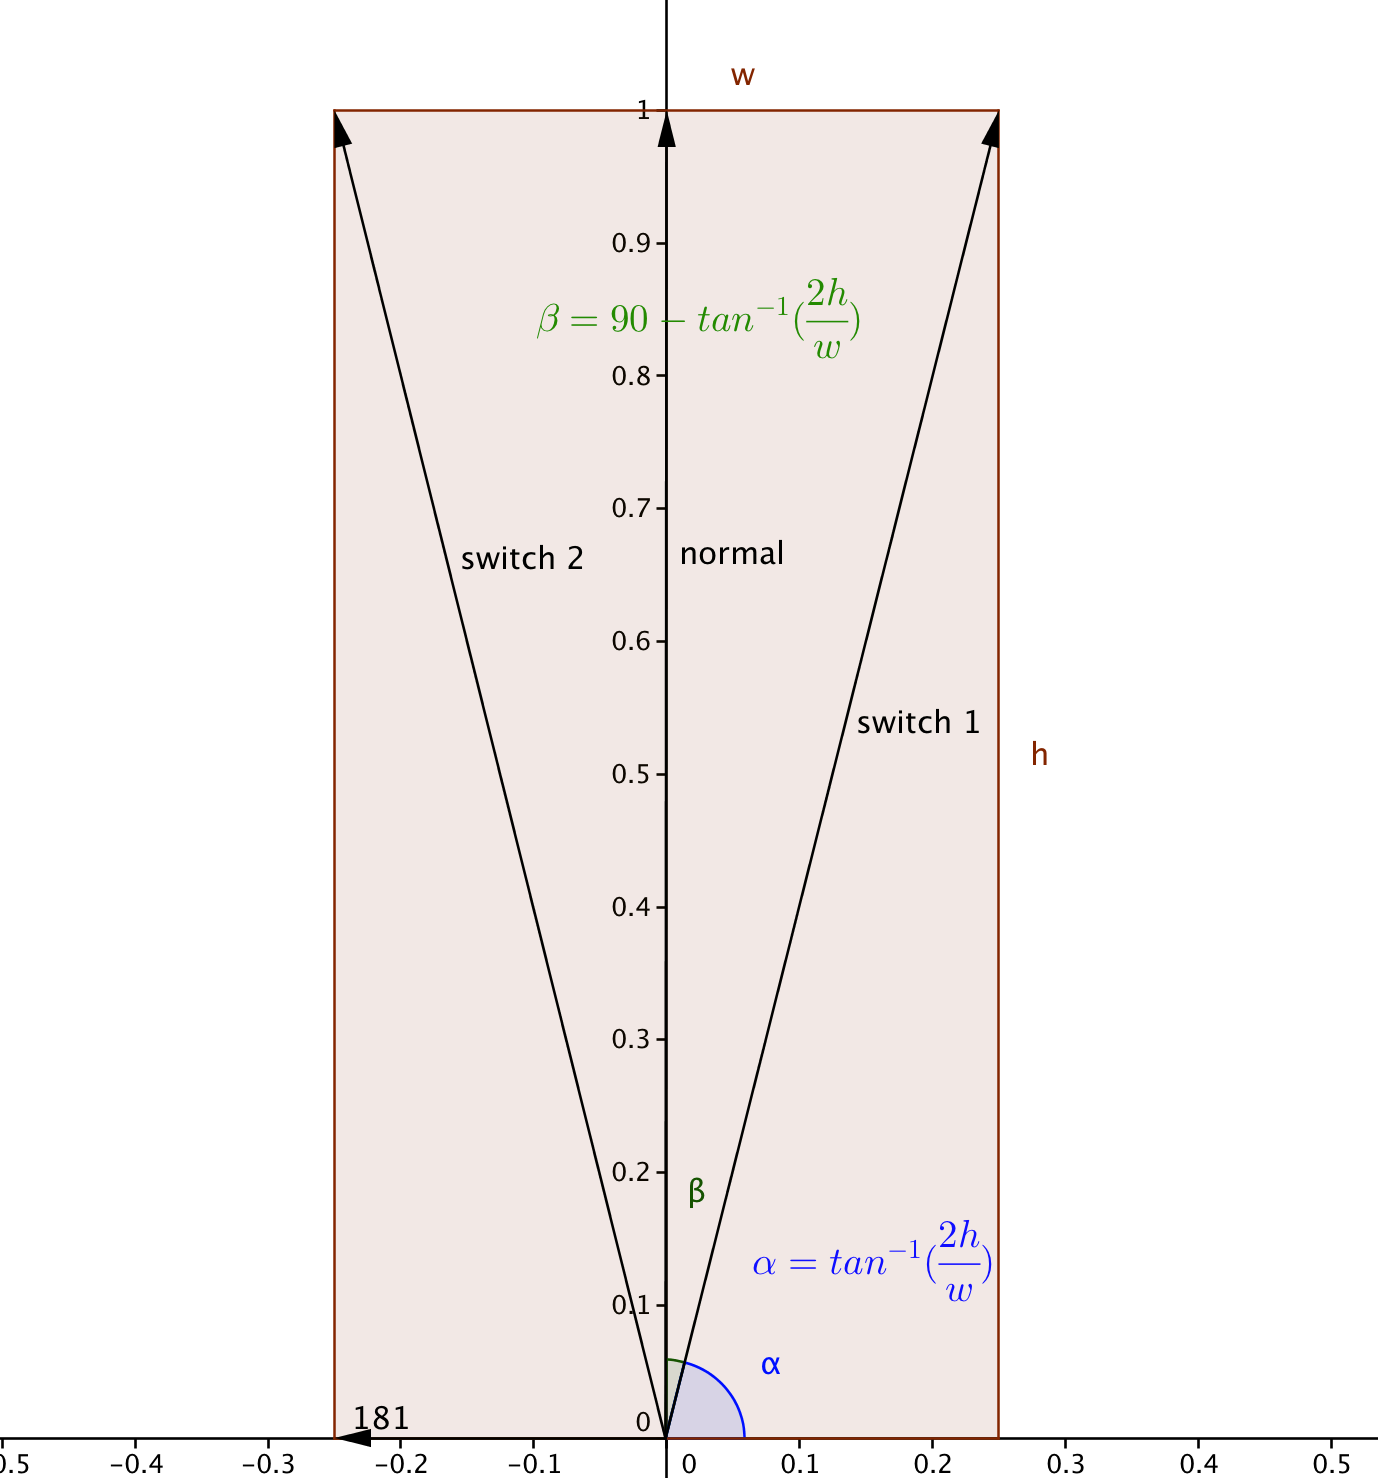
\includegraphics[height=4.5in]{look_ahead_bounding_box_transitions.png}
  \caption{Calculations for the transition angles}
\end{figure}
\FloatBarrier

This figure shows what how the transition angles are calculated.
After the ping corresponding to one of the transition angles is surpassed,
the calculations for the next set of pings switches between the two
equations shown in figure 3.

\subsection{Observations}

\subsubsection{Lidar Problems}
Because of the LIDAR's limited angular range, it is not very useful
for obstacle detection during turning.  The positioning of the LIDAR
unit prevents it from seeing obstacles to its side or behind it. While
we have the ability to decide if a turn is safe before we reaching the
starting point, we don't
have the ability to detect a new obstacle after the turn has started.

In addition we need to verify that the LIDAR gives consistent and
accurate data during turns.  The LIDAR method uses a rotating mirror
to send out and detect laser pings.\cite{deyle_sick_2008}
Theoretically the added rotation of the robot could ``smear'' the
LIDAR data.  Because we haven't used it during turns we have not
confirmed whether this is the case, but as we add the capabilities for
arcs this potential effect will become more important.

Another peculiarity of the LIDAR is the minimum range.  After an
object gets too close it disappears from the LIDAR.  This is most
likely because the circuitry of the LIDAR cannot detect the return
pulses fast enough to caclulate the data and so it filters them out.
Luckily it appears as if the minimum range is quite close. We found
the cutoff range to be around 0.1 m.

This range is not a problem from the robot's perspective because the
robot should never try to get close enough to object for this to
become an issue.  However, the opposite may not always be true. If the
robot stops for an approaching humand the human walks right up to the
robot without knowing the LIDAR limitations the robot may think the
human has disappeared and continue on its path.

The only potential solution we can see to this is to implement a
detection algorithm that examines where objects disappear, if the
object disappears by the robot's minimum range the robot can assume
the object is still there.  However, if the person leaves the range
while staying within the minimum range, the robot will think the human
is still there and wait forever. Obviously this is not ideal, however
other sensors like the Kinect camera will help us avoid this small, but potentially dangerous problem.

\subsubsection{Topic Name Change}
We noticed that the topic of the lidar data is different between the
simulator and the actual robot.  On the simulator the topic is
``base\_scan'' and on the robot it is ``base\_laser1\_scan''.  Currently
we make it easy to change the topic by modifying a constant at the top
of the source file.  However, this solution requires a recompilation
everytime the topic name is changed.

To solve this problem we are planning on implementing a new node
called topic\_translator.  This node will be responsible for
publishing everything it receives from base\_scan to
base\_laser1\_scan.  This node will only be run when testing via the
simulator.  This will prevent us from having to recompile everytime
the topic name changes.

The reason we are not planning on going the other way around and
translating from base\_laser1\_scan to base\_scan is because on the
actual robot we want as few nodes as possible to minimize the
possibility of a part failing.  In addition we can use the processor
cycles, memory and network bandwidth that would be used by the translator node on
other more interesting parts of the robot's software.

\subsection{Future Plans}
Currently the look ahead node only works for straight paths and arcs
of relatively low curvature.  In the future we would like to change
this so that the look ahead module works for arcs and potentially even
spins.

One way of doing this is to use the same bounding box algorithm to
calculate the distances for the box at different points along the
path.  After calculating the box, the box would be transformed back to
the robots coordinate system and compared with the LIDAR pings.

Another method would be to fatten the LIDAR pings and then make sure
the path segments don't pass through the englarged pings.  This is the
method we discussed in class.




